\section{Minimal-feedback experiment}\label{sec:minimal-experiment}
We test Proposition~\ref{prop:minimal-information} on the system in
Section~\ref{sec:neural-setup}, with $d\in\{8,32\}$, balls or boxes,
$R\in\{0.5,2\}$ and $m\in\{2,4\}$. The student is a bias-free
$d\to32\to m$ SiLU network followed by fixed orthonormal $P$.
Uniform scaling by latent Euclidean norm for balls or embedded maximum
absolute coordinate for boxes enforces feasibility while preserving
$\operatorname{range}(P)$. Parameters are float32; geometry and
coefficients are float64.

\subsection{Interfaces and protocol}
The 480-fit grid uses five seeds and six interfaces: target only
(set the unknown normal to zero), gain (one scalar per active target),
relevant ($r$ student-visible queries), random ($r$ ambient normal-space
queries with minimum-norm decoding), full face ($k$ normal-basis queries),
and privileged full information. Gain uses the minimum-norm normal
consistent with the response and known face. All methods fit
Eq.~\eqref{eq:minimal-loss}, normalized by $ad$.

Four direct controls are evaluated on all 80 caches: student basis,
random orthogonal student basis, hybrid, and pruned hybrid. The last
deletes normal coordinate directions orthogonal to the student and
student coordinate directions orthogonal to the normal space, then
chooses the smaller remaining basis. It does not combine linearly
dependent directions. Direct controls add 80 fits using the original
five paired seeds in four representative conditions
(Table~\ref{tab:direct-training}). These conditions were chosen after
inspection of the grid; they check interface fidelity and are not an
independent performance confirmation.

Another 40 fits use five new seeds, eight interfaces (the four direct
controls plus target, relevant, full face and full information), and
Eq.~\eqref{eq:shared-actuation} with $d=8,m=4,R=0.5$. The first three
initial coordinates have independent random signs and magnitudes
uniform on $[6,10]$; the others are uniform on $[-0.1,0.1]$. All 12
teacher states have exactly those three active coordinates. This is a
constructed shared-actuation test of $k=3,m=4,r=1$, not a naturally
occurring benchmark. A latent rotation makes all student axes visible.

Protocols, seeds and numerical-source hashes are fixed before their
respective fits. The primary checks exact coefficient recovery to
relative RMS tolerance $10^{-9}$ and actual scalar query counts.
Secondary regret fidelity uses tolerance $10^{-3}$ per pair against
full information, without a population equivalence claim. All 600
fits are retained. The scalar oracle excludes shared target/baseline
preparation; full-vector derivatives use a different interface.
The analytic coefficient is hidden by experimental restriction only.

\subsection{Results}
All coefficient and count checks pass. The 480-fit grid reproduces
full-information regret within $3.81\times10^{-12}$ in all 80 pairs.
All 120 additional checkpoints pass independent re-evaluation; the
110 exact-recovery/full-information comparisons differ in regret by
at most $8.04\times10^{-13}$ and in closed-loop cost by
$2.83\times10^{-11}$. The maximum coefficient error across all direct
checks is $3.56\times10^{-15}$. This is the expected consequence of
preserving the objective, not evidence of a better optimizer.

Every random-embedding cache has $r=\min(k,m)$. In the box caches,
relevant, hybrid and pruned hybrid each use 332,362 responses; student
basis and its orthogonal rotation use 444,234; full face uses 1,039,456.
Thus the 68.03\% reduction against full-face recovery is shared by the
simple hybrid. Relevant queries save 25.18\% against the direct student
basis and \emph{nothing against hybrid}. Ball counts likewise match
hybrid. The ambient-random baseline's failures do not extend to a
complete orthogonal student-space basis.

In the shared-actuation construction, all 61,440 cached states have
$k=3,m=4,r=1$. Relevant feedback uses one query per state, hybrid and
pruned hybrid three, and either student basis four
(Figure~\ref{fig:direct-query}). Every recovery method yields mean
regret 0.523674 and mean closed-loop cost 189.698903, versus 0.627840
and 190.883229 for target-only fitting. The extra saving depends on
linear dependence among visible directions, not simply zero-coordinate
pruning. The construction establishes this possibility, not its
prevalence in applications.
\begin{figure}[htbp]\centering
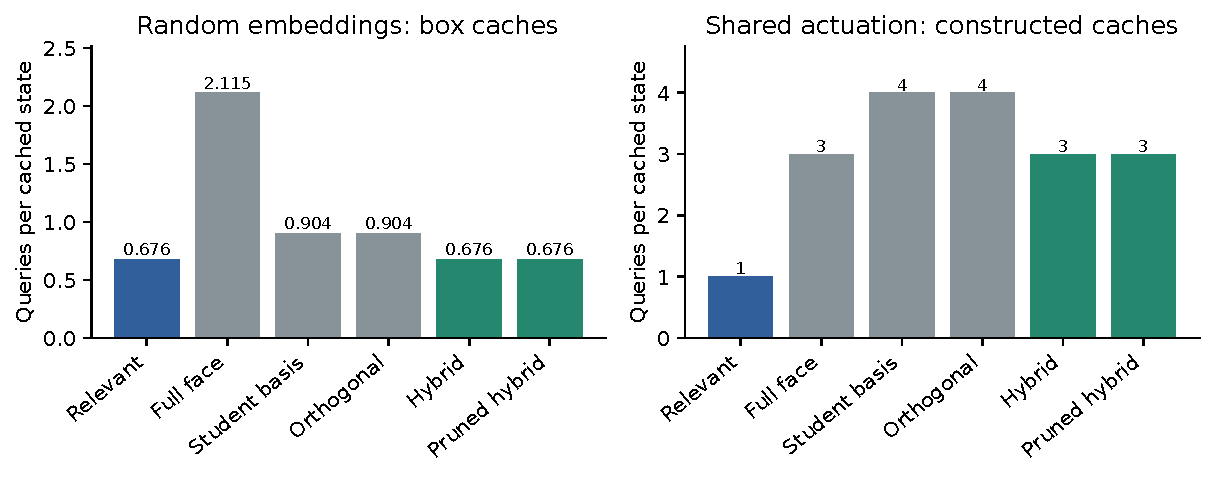
\includegraphics[width=\linewidth]{figures/direct_query_controls.pdf}
\caption{Direct controls separate dimension reduction from additional
alignment. Counts include inactive targets. Left: all random-embedding
box caches; relevant and hybrid coincide. Right: a constructed shared
actuation geometry; every state has positive rank one.}
\label{fig:direct-query}
\end{figure}
\begin{table}[htbp]\centering\small
\caption{Additional interface checks: means over five paired seeds. All exact-recovery interfaces agree to the reported precision; full-reference values are shown. These checks reuse four conditions and add a constructed shared-actuation condition.}\label{tab:direct-training}
\begin{tabular}{lrrrr}\toprule
Condition & Fits & Regret & Cost & Max. $|\Delta\mathcal R|$\\\midrule
box, $d=8,m=2,R=0.5$ & 20 & 0.585439 & 8.101119 & $0$\\
box, $d=32,m=2,R=0.5$ & 20 & 0.900619 & 15.475675 & $0$\\
box, $d=32,m=4,R=2$ & 20 & 0.820332 & 15.014408 & $0$\\
ball, $d=32,m=4,R=0.5$ & 20 & 0.715371 & 15.313708 & $8.03\times10^{-13}$\\
Shared actuation & 40 & 0.523674 & 189.698903 & $0$\\
\bottomrule\end{tabular}
\end{table}


Timing includes geometry, query construction, actual responses and
decoding on 12,288-state batches, after one warmup and with three
shuffled repeats. Median batch times on random box caches are 1.348\,ms
for relevant, 0.753\,ms for student basis and 0.890\,ms for hybrid;
on structured caches they are 2.268, 0.879 and 0.802\,ms. With this cheap
analytic oracle, rank construction costs more than the saved responses.
These implementation measurements do not support a runtime advantage.

The complete grid, including gain/random failures and uncertain
target-only comparisons, is in \ref{app:minimal-grid} and
\ref{app:minimal-comparisons}. A further 2,304 algebraic checks verify
Eq.~\eqref{eq:truncated-feedback}: arbitrarily small perturbations can
raise exact rank from one to three, while one-query approximation error
changes continuously with the omitted singular values
(\ref{app:approximate-feedback}). No noisy neural training is claimed.

